\documentclass[UTF8,zihao=-4]{ctexart}

\usepackage[a4paper,top=2.5cm,bottom=2.5cm,left=2.6cm,right=2.6cm]{geometry}
\usepackage{graphicx}
\usepackage{float}
\usepackage{booktabs}
\usepackage{tabularx}
\usepackage{enumitem}
\usepackage{caption}
\usepackage{xcolor}
\usepackage{hyperref}
\usepackage{fancyhdr}
\usepackage{titlesec}
\usepackage{setspace}

\graphicspath{{latex_figures/}}
\hypersetup{
  colorlinks=true,
  linkcolor=black,
  urlcolor=teal
}

\definecolor{nstiGreen}{HTML}{1F6F5B}
\definecolor{nstiDark}{HTML}{14352F}
\definecolor{nstiLight}{HTML}{EFF7F3}

\titleformat{\section}{\Large\bfseries\color{black}}{\thesection}{0.8em}{}
\titleformat{\subsection}{\large\bfseries\color{black}}{\thesubsection}{0.8em}{}
\titleformat{\subsubsection}{\normalsize\bfseries\color{black}}{\thesubsubsection}{0.8em}{}
\captionsetup{font=small,labelfont=bf}
\setlist[itemize]{leftmargin=2em,itemsep=0.25em,topsep=0.3em}
\setlist[enumerate]{leftmargin=2.2em,itemsep=0.25em,topsep=0.3em}
\linespread{1.25}

\pagestyle{fancy}
\setlength{\headheight}{15pt}
\fancyhf{}
\fancyhead[L]{NSTI 应用案例说明}
\fancyhead[R]{人工智能辅助学习实践}
\fancyfoot[C]{\thepage}

\begin{document}

\begin{titlepage}
  \centering
  \vspace*{2.2cm}
  {\Huge\bfseries 基于人工智能辅助的校园偏好测评工具设计与实现\par}
  \vspace{0.8cm}
  {\Large 以 NSTI（NNU Student Type Indicator）项目为例\par}
  \vspace{2.0cm}
  
\includegraphics[width=0.78\textwidth]{nsti_logo_horizontal.png}
  \vspace{2.2cm}
  \makebox[\textwidth][c]{\Large\bfseries 应用案例说明}\par
  \vspace{0.5cm}
  {\large 2026 年 4 月\par}
  \vspace*{1.6cm}
\end{titlepage}

\tableofcontents
\newpage

\section{任务背景}

做 NSTI 的起点，并不是想再做一个“校园版 MBTI”。我最早注意到的是一个很普通的现象：同学们愿意聊人格测试，也愿意把测试结果拿来做社团破冰、聊天开场或自我介绍，但很多结果离校园生活太远。大家记住了几个字母，却很难说清这些字母和自己在图书馆、校车、宿舍、小组作业中的真实状态有什么关系。

因此，我想把测评的重点从抽象人格转向具体校园经验。NSTI 的全称是 NNU Student Type Indicator，它围绕南京师范大学学生熟悉的学习、通勤、协作、社交和校园停留场景展开，希望用更贴近本校生活的语言，描述一个人在校园里的偏好和节奏。它不是心理诊断，也不用于能力评价，而是一个偏轻量的校园偏好画像工具。

这个项目同时也是一次人工智能辅助学习实践。这里需要说明的是，我主要依赖的不是单纯的网页端聊天工具，而是 OpenAI Codex 这一类运行在编辑器和本地项目环境中的 agent。网页端 ChatGPT、Gemini 更适合讨论想法、回答问题或生成一段参考文字；Codex 这类 agent 则可以读取项目文件、理解仓库结构、修改代码和文档、运行命令，并根据运行结果继续调整。对我来说，它更像一个能进入项目现场的协作者，而不是只停留在聊天窗口里的回答者。

我的实际做法是：先由我确定创意边界和项目方向，再用自然语言把需求、审美倾向和具体限制说清楚；随后借助模型把这些想法整理成更准确的提示词或任务说明，交给 Codex 这样的编辑器 agent 去执行。它可以把任务落实到代码、页面、文档和配图生成脚本里，我再对结果进行筛选、修改和验收。因此，NSTI 并不是 AI 自动生成的作品，而是一次“人提出创意与判断，agent 承担执行和迭代”的协作实践。

\section{任务目标}

本项目主要完成三件事：

\begin{enumerate}
  \item 设计一套贴近南京师范大学校园生活的偏好测评体系，避免直接照搬现成的人格测试框架。
  \item 做出一个可以实际访问和使用的网页工具，形成“作答、计算、展示结果”的完整流程。
  \item 把 AI 在项目中的真实使用方式整理成案例材料，便于展示、复盘和提交。
\end{enumerate}

\begin{figure}[H]
  \centering
  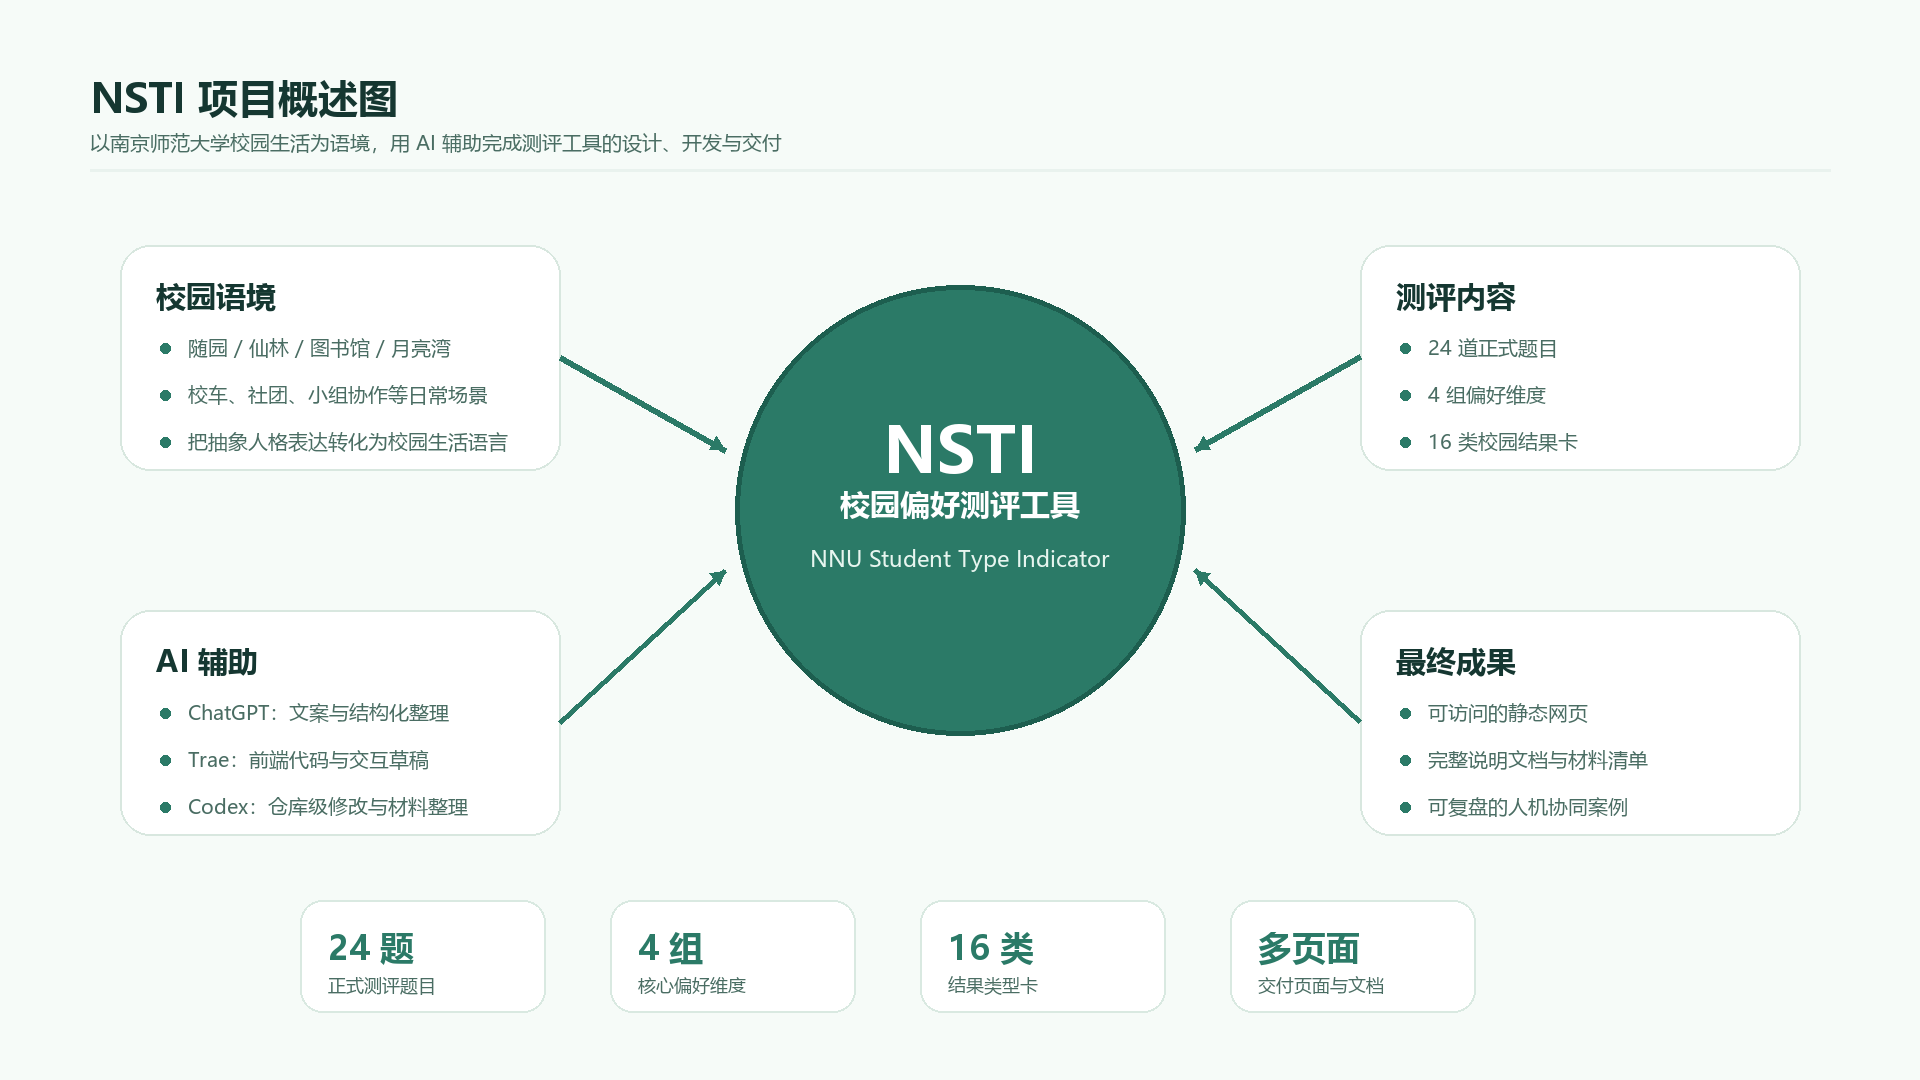
\includegraphics[width=\textwidth]{fig4_overview.png}
  \caption{NSTI 项目概述图}
\end{figure}

\section{工具、模型与 Skills 使用}

本项目没有只依赖一个聊天窗口，而是以 OpenAI Codex 这类编辑器 agent 为主，再配合通用大语言模型、前端开发工具和部署工具。这样安排是因为 NSTI 不只是写一段文案，还要在真实仓库里处理题库、页面、样式、脚本、说明文档和 PDF 材料。网页端问答工具可以帮我把问题想清楚，或者先写出一段参考内容；但真正要改文件、跑脚本、查编译结果时，还是需要 Codex 进入本地项目环境去完成。

\subsection{主要工具分工}

\begin{table}[H]
  \centering
  \caption{项目中使用的主要工具及作用}
  \renewcommand{\arraystretch}{1.35}
  \setlength{\extrarowheight}{3pt}
  \begin{tabularx}{\textwidth}{>{\raggedright\arraybackslash\bfseries}p{3.6cm}>{\raggedright\arraybackslash}X}
    \toprule
    工具 & 使用方式 \\
    \midrule
    网页端通用模型 & 包括 ChatGPT、Gemini 等。主要用于讨论想法、拆解问题、改写局部文案和生成参考表达。它们更像可以反复交流的文字与研究助手，适合帮助我把模糊想法说清楚，但通常不直接接触本地项目文件。 \\
    Trae & 用于前端开发过程中的代码补全、HTML/CSS/JavaScript 草稿生成、局部样式调整和交互逻辑排查。它适合在编辑器里快速试方案。 \\
    OpenAI Codex & 本项目的主要 AI 工具。它作为编辑器和本地仓库中的 agent 使用，负责读取项目上下文、理解文件结构、修改 HTML/CSS/JavaScript 与 Markdown/LaTeX 文档、运行生成脚本和编译命令，并根据运行结果继续迭代。 \\
    Git / GitHub & 用于版本管理、文件归档和代码托管，使项目修改过程有记录可查。 \\
    Vercel & 用于静态站点部署和线上访问验证，使项目从本地页面变成可以展示的网页成果。 \\
    高德地图、天气等开放能力 & 用于“关于随园”等扩展页面，让网站不止停留在测评本身，也带一点校园生活服务和文化表达。 \\
    \bottomrule
  \end{tabularx}
\end{table}

\subsection{使用模型说明}

内容整理和中文表达会参考 GPT-4o / GPT 系列通用模型；仓库阅读、文件修改和工程化整理则主要依赖 GPT-5 / Codex 系列代码模型。这里的区别不只是模型名称不同，而是使用场景不同：网页端模型更多用于讨论和提示词整理，Codex 则作为 agent 接收这些任务说明，进入项目环境中连续操作。Trae 中的 AI 编程模型主要用于编辑器内的前端代码生成和局部调试，属于快速试方案的辅助工具。

\subsection{Skills 与能力模块}

这里所说的 Skills，并不是单独的某一个软件，而是 AI agent 在执行任务时可以调用或复用的能力模块。它更接近一套被整理好的工作流：例如遇到前端页面问题时，调用前端开发与浏览器验证能力；遇到提交材料问题时，调用 Markdown/LaTeX 文档整理能力；遇到部署问题时，调用 Vercel 与项目交付能力。这样做的好处是，任务不会停留在一次性的聊天回答里，而是能被拆成更稳定、更可检查的执行步骤。

实际使用时，我把项目拆成若干小任务，而不是一次性让 AI 生成整个作品。比较常见的流程是：我先描述目标，例如“把这段材料写得更像真实项目复盘”“把工具部分补充 Codex 和网页端模型的区别”“重新生成一张更清楚的流程图”；随后让模型把需求整理成更准确的提示词或任务清单，再交给 Codex 在项目文件中实施。涉及的能力模块包括前端开发、Markdown 文档整理、浏览器验证、Vercel 部署、资料结构化和可视化辅助。这样拆分之后，每一步都更容易检查，也更容易发现不合适的内容。

\begin{figure}[H]
  \centering
  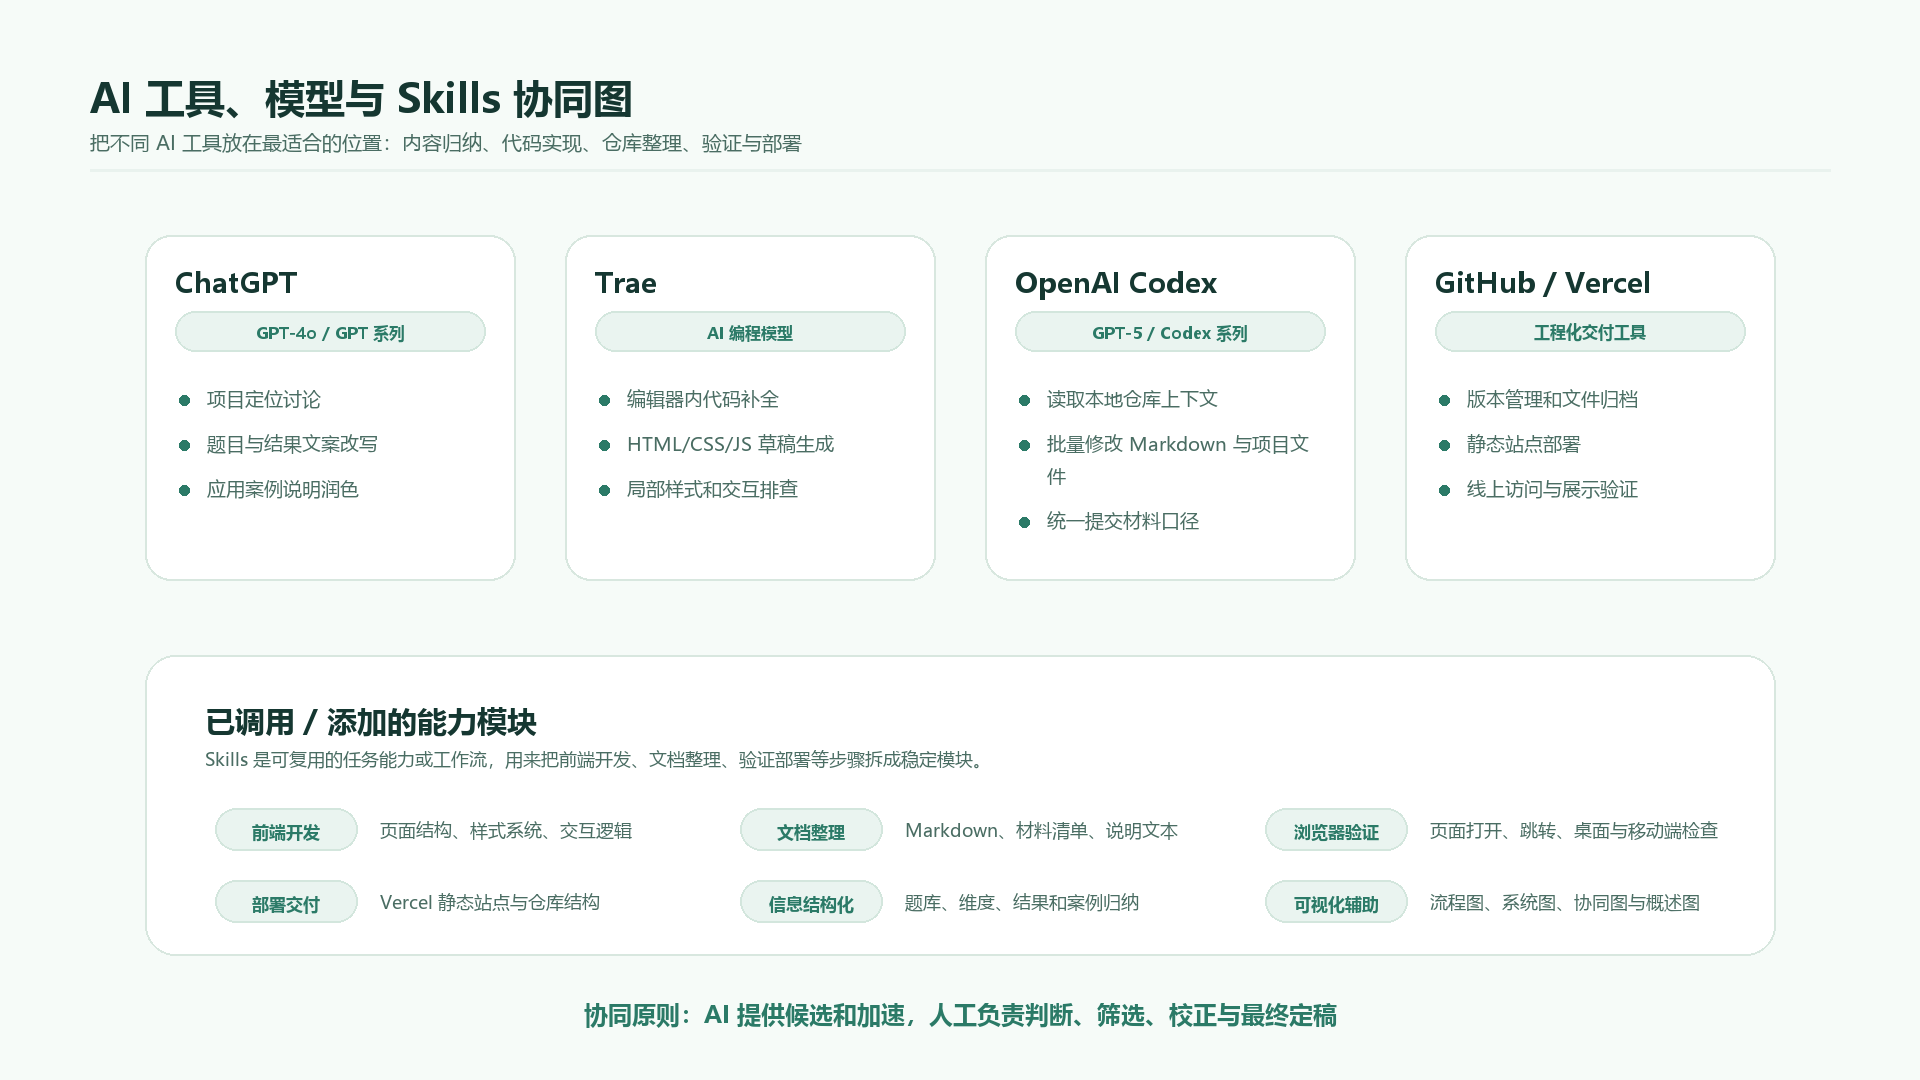
\includegraphics[width=\textwidth]{fig6_ai_tools.png}
  \caption{AI 工具、模型与 Skills 协同图}
\end{figure}

\section{技术路线}

NSTI 的技术路线可以概括为四个层次：内容模型设计、测评逻辑设计、静态前端实现和线上部署交付。

\subsection{内容模型设计}

项目先确定“校园偏好测评”这一边界，再围绕学习节奏、空间偏好、协作方式、社交状态等校园生活维度设计题目。题目的生活化方向主要来自我对校园场景的观察和筛选；AI 更多是在已有方向上帮我整理资料、提供表达备选。至于一句题目像不像南师大学生真实会遇到的情境，仍然需要我自己判断。

\subsection{测评逻辑设计}

项目采用多题目、多维度累积分值的方式，把用户选项映射到不同偏好维度，再根据得分组合生成结果类型。与直接输出 MBTI 字母不同，NSTI 更强调“校园锚点 + 场景解释 + 行动建议”，让结果更容易被理解和讨论。

\subsection{前端工程实现}

网页主体使用 HTML、CSS 和 JavaScript 构建，包含首页、答题页、结果页、题库说明、评价体系、隐私与免责声明、结果图鉴和随园扩展页面。JavaScript 负责题目切换、答案记录、进度显示、得分计算和结果匹配；CSS 负责绿色视觉体系、响应式布局和移动端适配。

\subsection{部署与交付}

项目通过 Git/GitHub 管理文件，通过 Vercel 部署为静态站点，并整理出 Markdown 正文、LaTeX 说明文档、材料清单和配图文件。这样既能展示网页成果，也能把我的设计、开发和 AI 辅助过程说清楚。

\begin{figure}[H]
  \centering
  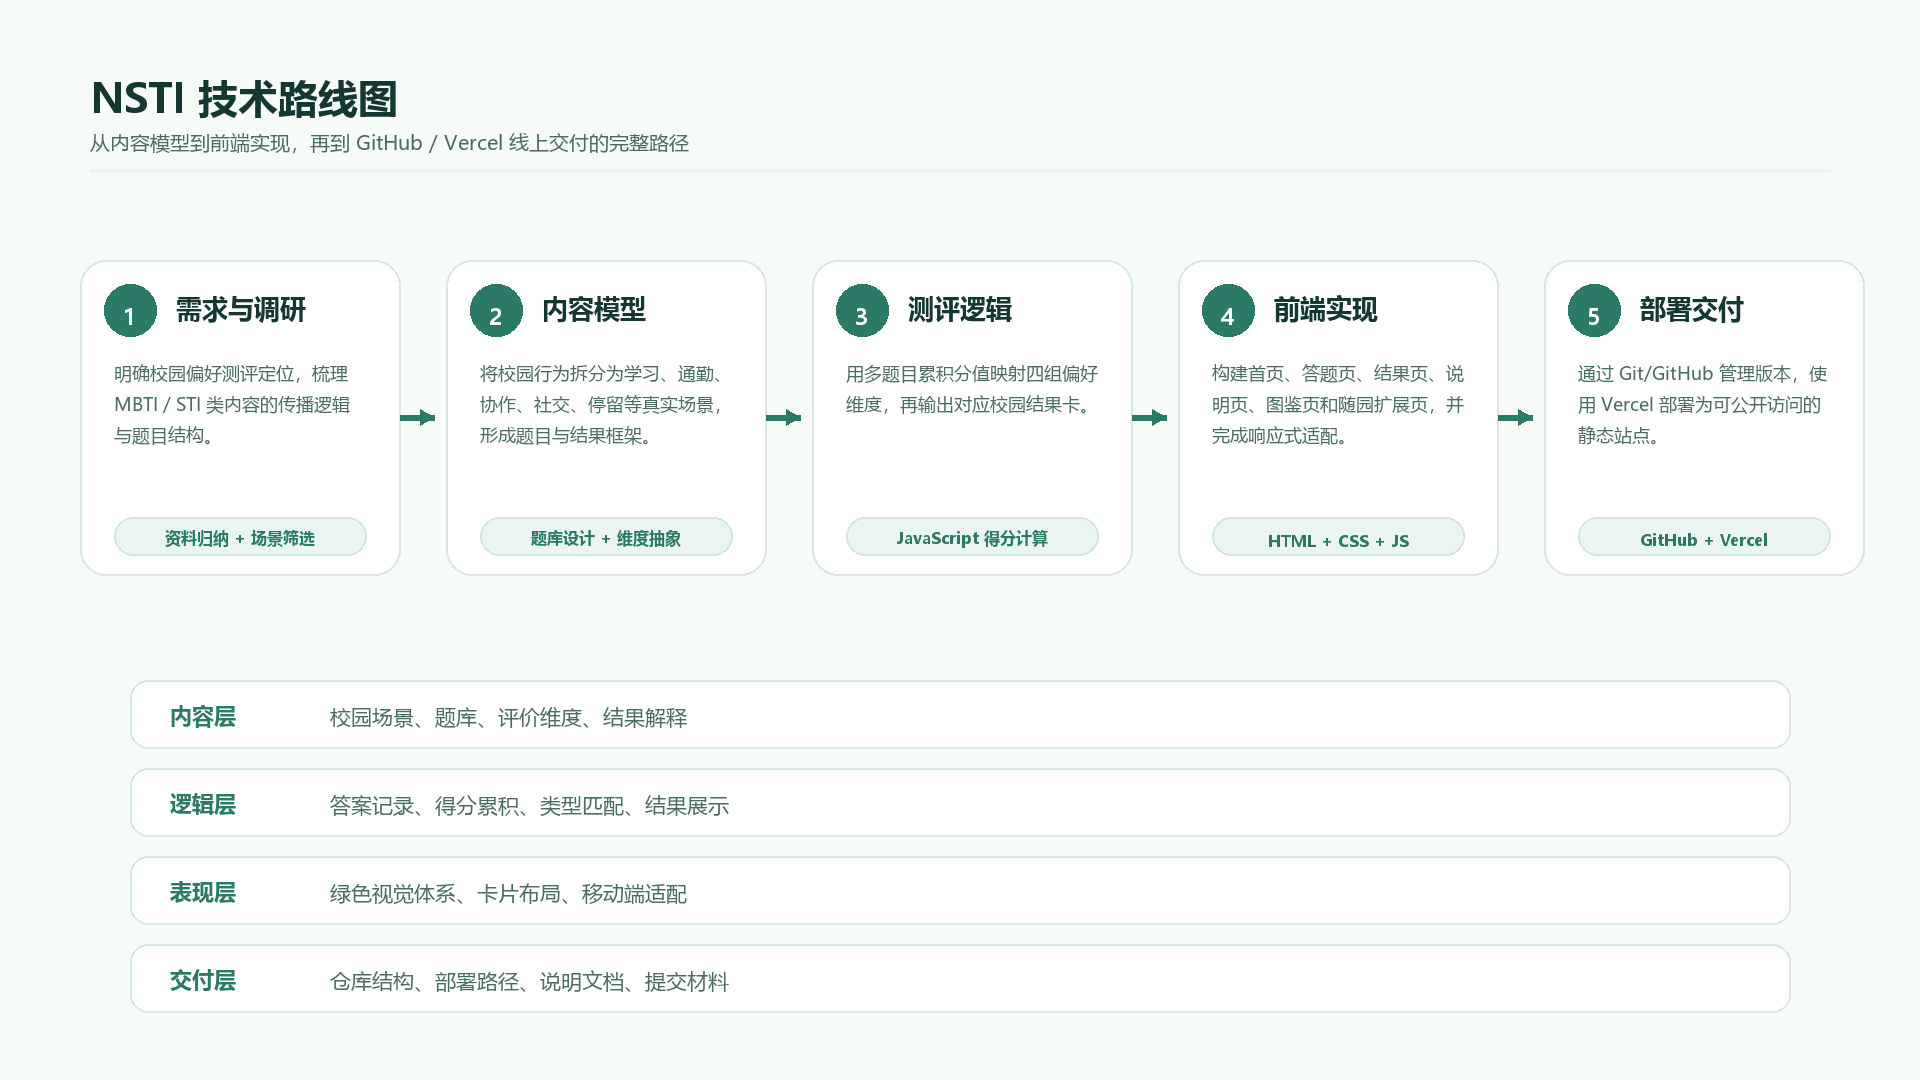
\includegraphics[width=\textwidth]{fig5_technical_route.png}
  \caption{NSTI 技术路线图}
\end{figure}

\section{应用全过程}

\subsection{问题提出与项目立项}

项目最初来自一个很小的观察：很多测试结果能让人一眼记住标签，却不一定能解释一个人在校园里怎么学习、怎么赶路、怎么和人合作。于是我把 NSTI 定位为校园偏好画像工具，而不是通用人格测试。它关心的不是“你是哪一种人”，而是“你在南师这样的校园里，通常以什么节奏生活和行动”。

在立项阶段，我主要是先自己查找和阅读人格测试、STI 类测试的定义说明，以及公开题库中的部分样题，观察这些题目通常怎样把一个抽象偏好转化为具体选择。随后，我把注意力转回南师大的真实生活场景，围绕图书馆、自习、校车、宿舍、小组作业、社团活动等经验，先提出了一批生活化题目的构想。也就是说，NSTI 的题目方向和校园场景不是由 AI 替我决定的，而是我在调研、观察和筛选之后自己收束出来的。

\begin{figure}[H]
  \centering
  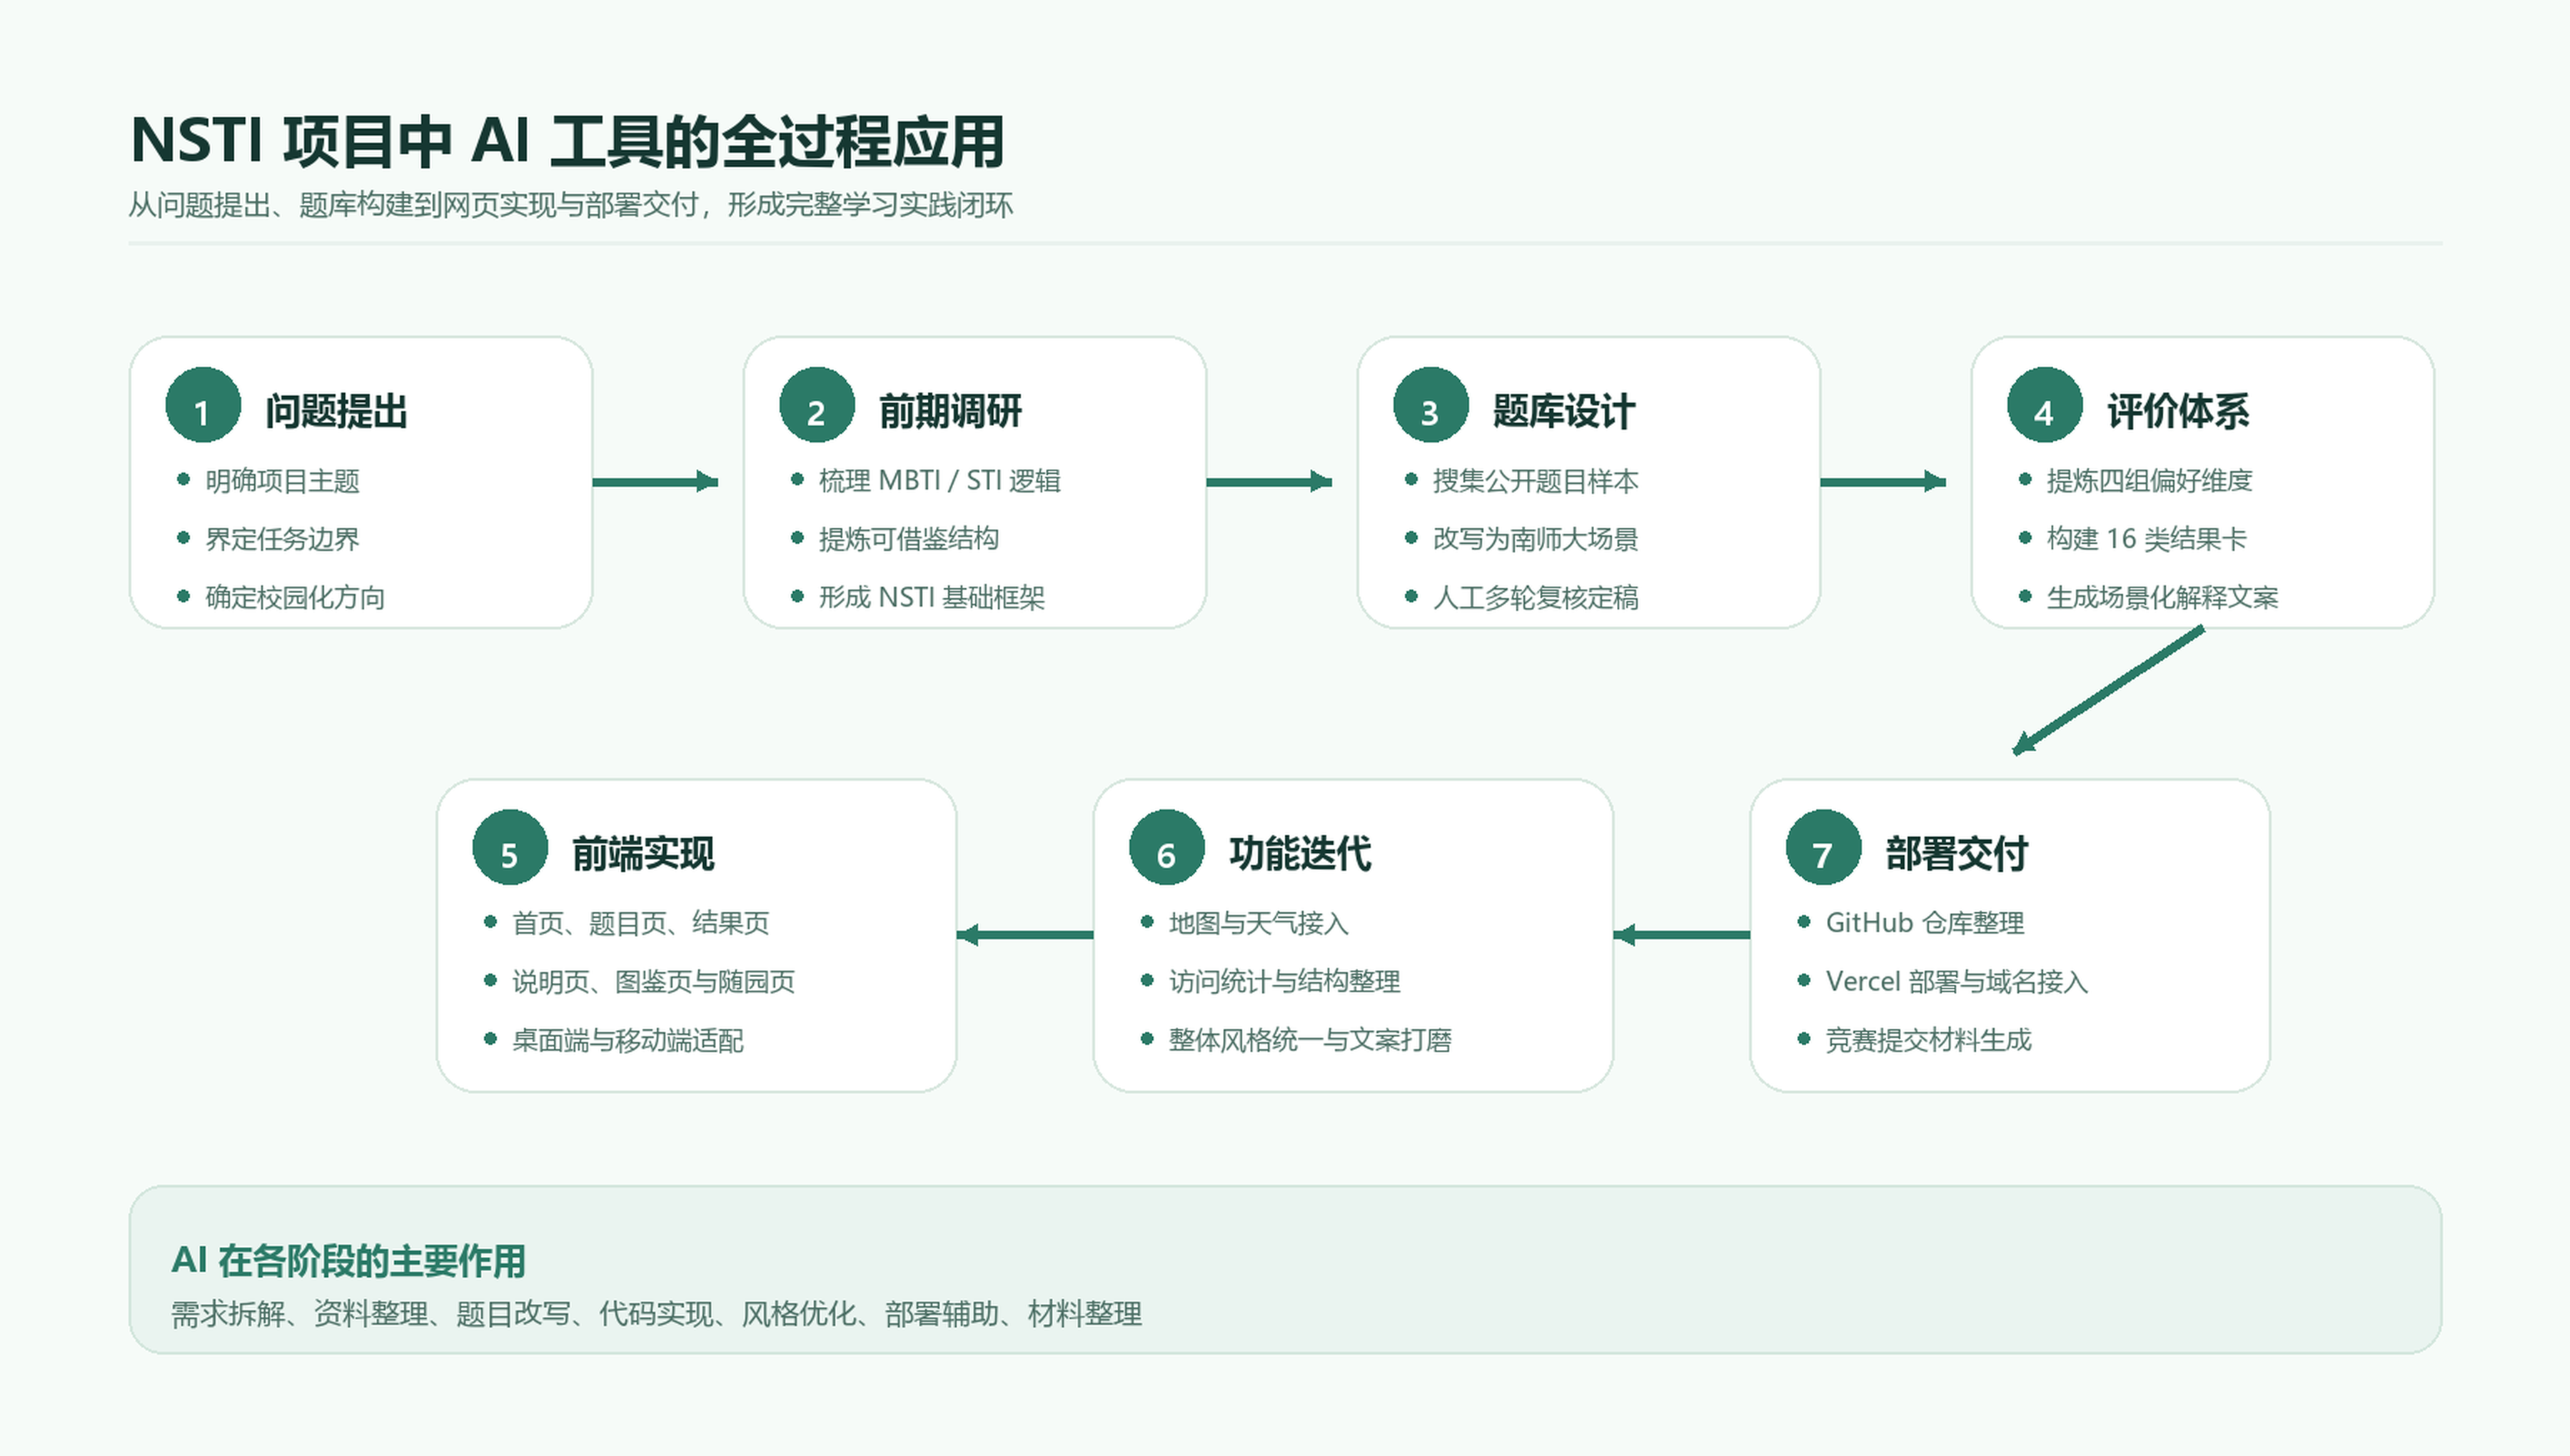
\includegraphics[width=\textwidth]{fig1_ai_process_hires.png}
  \caption{NSTI 项目中 AI 工具的全过程应用}
\end{figure}

\subsection{前期调研与框架整理}

正式写题目之前，我先研究了网络上常见的人格测试和 STI 类内容。调研重点不是复制题目，而是看清它们为什么容易传播、题目如何对应维度、结果为什么容易被社交讨论。AI 在这里主要用于资料归纳和逻辑整理，帮我更快看出“多道题对应若干维度，再根据累积分值输出类型”的基本结构。

在这个基础上，我没有沿用 MBTI 的原始字母作为主结果，而是把 NSTI 明确为“校园行为偏好工具”。这个边界很重要，因为它决定了后续文案不能写得像心理测验，更不能让用户误以为结果具有诊断意义。

\subsection{题库搜集、筛选与校园化改写}

题库是整个项目里最费时间的部分。我采用的是“公开题库逻辑参考 + 校园场景重写”的方法：先看题目背后的判断逻辑，再把它改写成南师大学生更熟悉的情境。

例如，抽象的“偏好安静还是热闹”可以改成图书馆、敬文广场、社团活动或宿舍群聊中的选择；抽象的“计划性”可以放进小组作业、赶校车、复习安排等场景中。这样的改写会让作答更自然，也能让结果解释更有校园感。

AI 在这一阶段提供过不少候选表达，但我做了多轮人工复核。重点检查四件事：题目是否对应维度，选项是否暗含价值高低，校园地标和称呼是否真实，句子是否生硬或不符合学生日常表达。最终题库定为 24 道题，覆盖 4 组偏好维度，每组 6 道题，作答形式为单题 4 选 1。

\subsection{评价体系设计}

NSTI 的评价体系由四组偏好维度构成：能量补给、观察视角、逻辑基准和生活步调。这四个维度不是从某个模型直接搬来的，而是从校园生活中常见的差异里提炼出来的。

为了降低“像 MBTI 换皮”的感觉，我后来又调整了结果形式：不再把字母组合放在最前面，而是采用校园锚点、场景化描述和地标命名。这样结果读起来更像一份校园生活图鉴，而不是一张抽象类型表。

\begin{figure}[H]
  \centering
  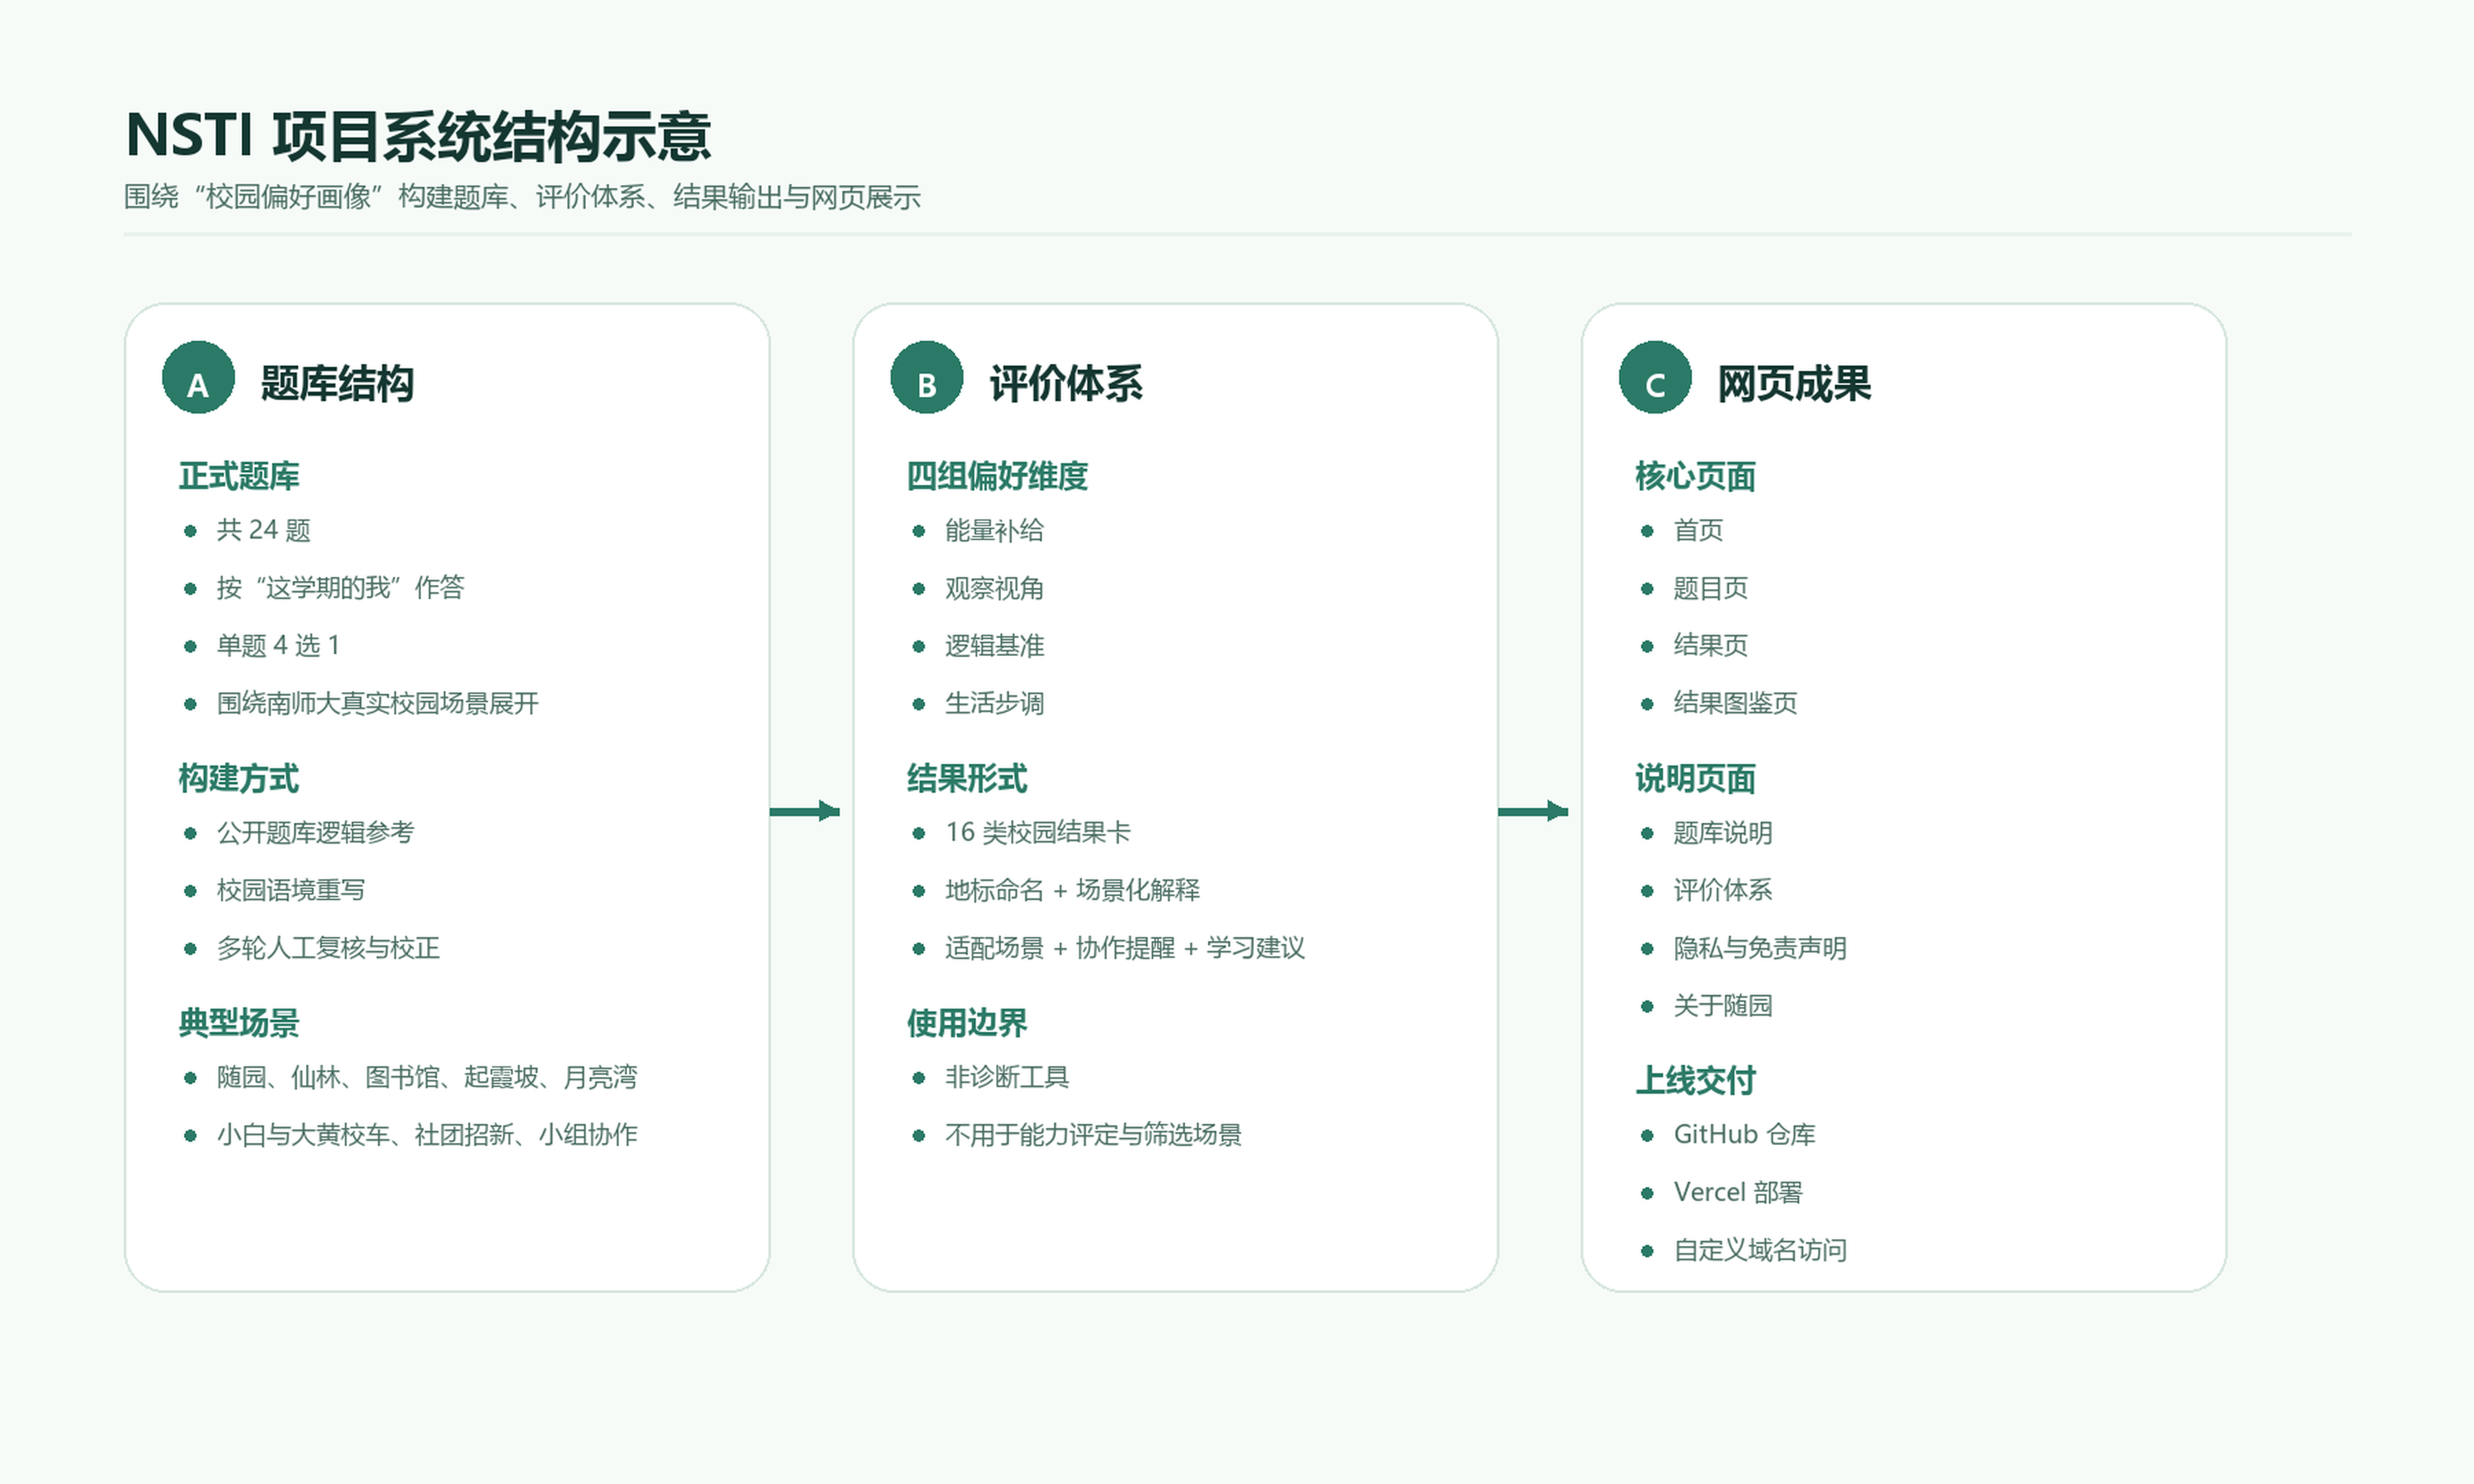
\includegraphics[width=\textwidth]{fig2_system_structure_hires.png}
  \caption{NSTI 系统结构示意}
\end{figure}

\subsection{前端页面设计与交互实现}

内容框架确定后，我开始做网页。项目采用静态前端形式，主要由 HTML、CSS 和 JavaScript 组成。这样部署简单，访问也轻量，适合课程项目和竞赛展示。

站点包括首页、题目页、结果页、题库说明、评价体系、隐私与免责声明、结果图鉴和“关于随园”等页面。AI 在这一阶段主要参与页面结构草稿、CSS 样式组织、题目切换逻辑、进度条、得分计算和跳转问题排查。我自己主要负责视觉取舍和最终体验判断，比如首页不要堆太多解释，主色调要更接近南师大的绿色印象，手机端不能出现错位。

\subsection{扩展内容与上线整理}

主测评页面完成后，我又扩展了“关于随园”页面，加入地标、地图和天气信息。这个部分不是测评逻辑的核心，但能让项目从单一测试页延伸到校园文化表达。

后续工作包括接入高德地图与天气能力、增加结果图鉴、接入 Vercel Analytics、整理目录结构、清理无用文件，并把项目整理为可部署的 GitHub 仓库和 Vercel 静态站点。到这一步，NSTI 已经不只是一个页面草稿，而是从选题、调研、题库、评价体系、前端实现到提交材料都能对应起来的完整作品。

\subsection{人机协同方式}

这次项目让我最有感触的一点是：Codex 这类 agent 可以明显加快进度，甚至可以连续完成“读文件、改代码、生成图片、编译 PDF”这样的流程，但它不能替我判断“像不像南师大”。题目里的地标、称呼、生活节奏，结果页的语气，免责声明的边界，都需要我反复看、反复改。

所以本项目更接近一种“人提出创意和边界，模型帮助整理提示词，Codex 进入项目执行，人再判断和修正”的协作方式。AI 和 agent 负责提高推进速度，我负责判断哪些内容真的适合 NSTI，哪些内容需要删掉或重写。

\begin{figure}[H]
  \centering
  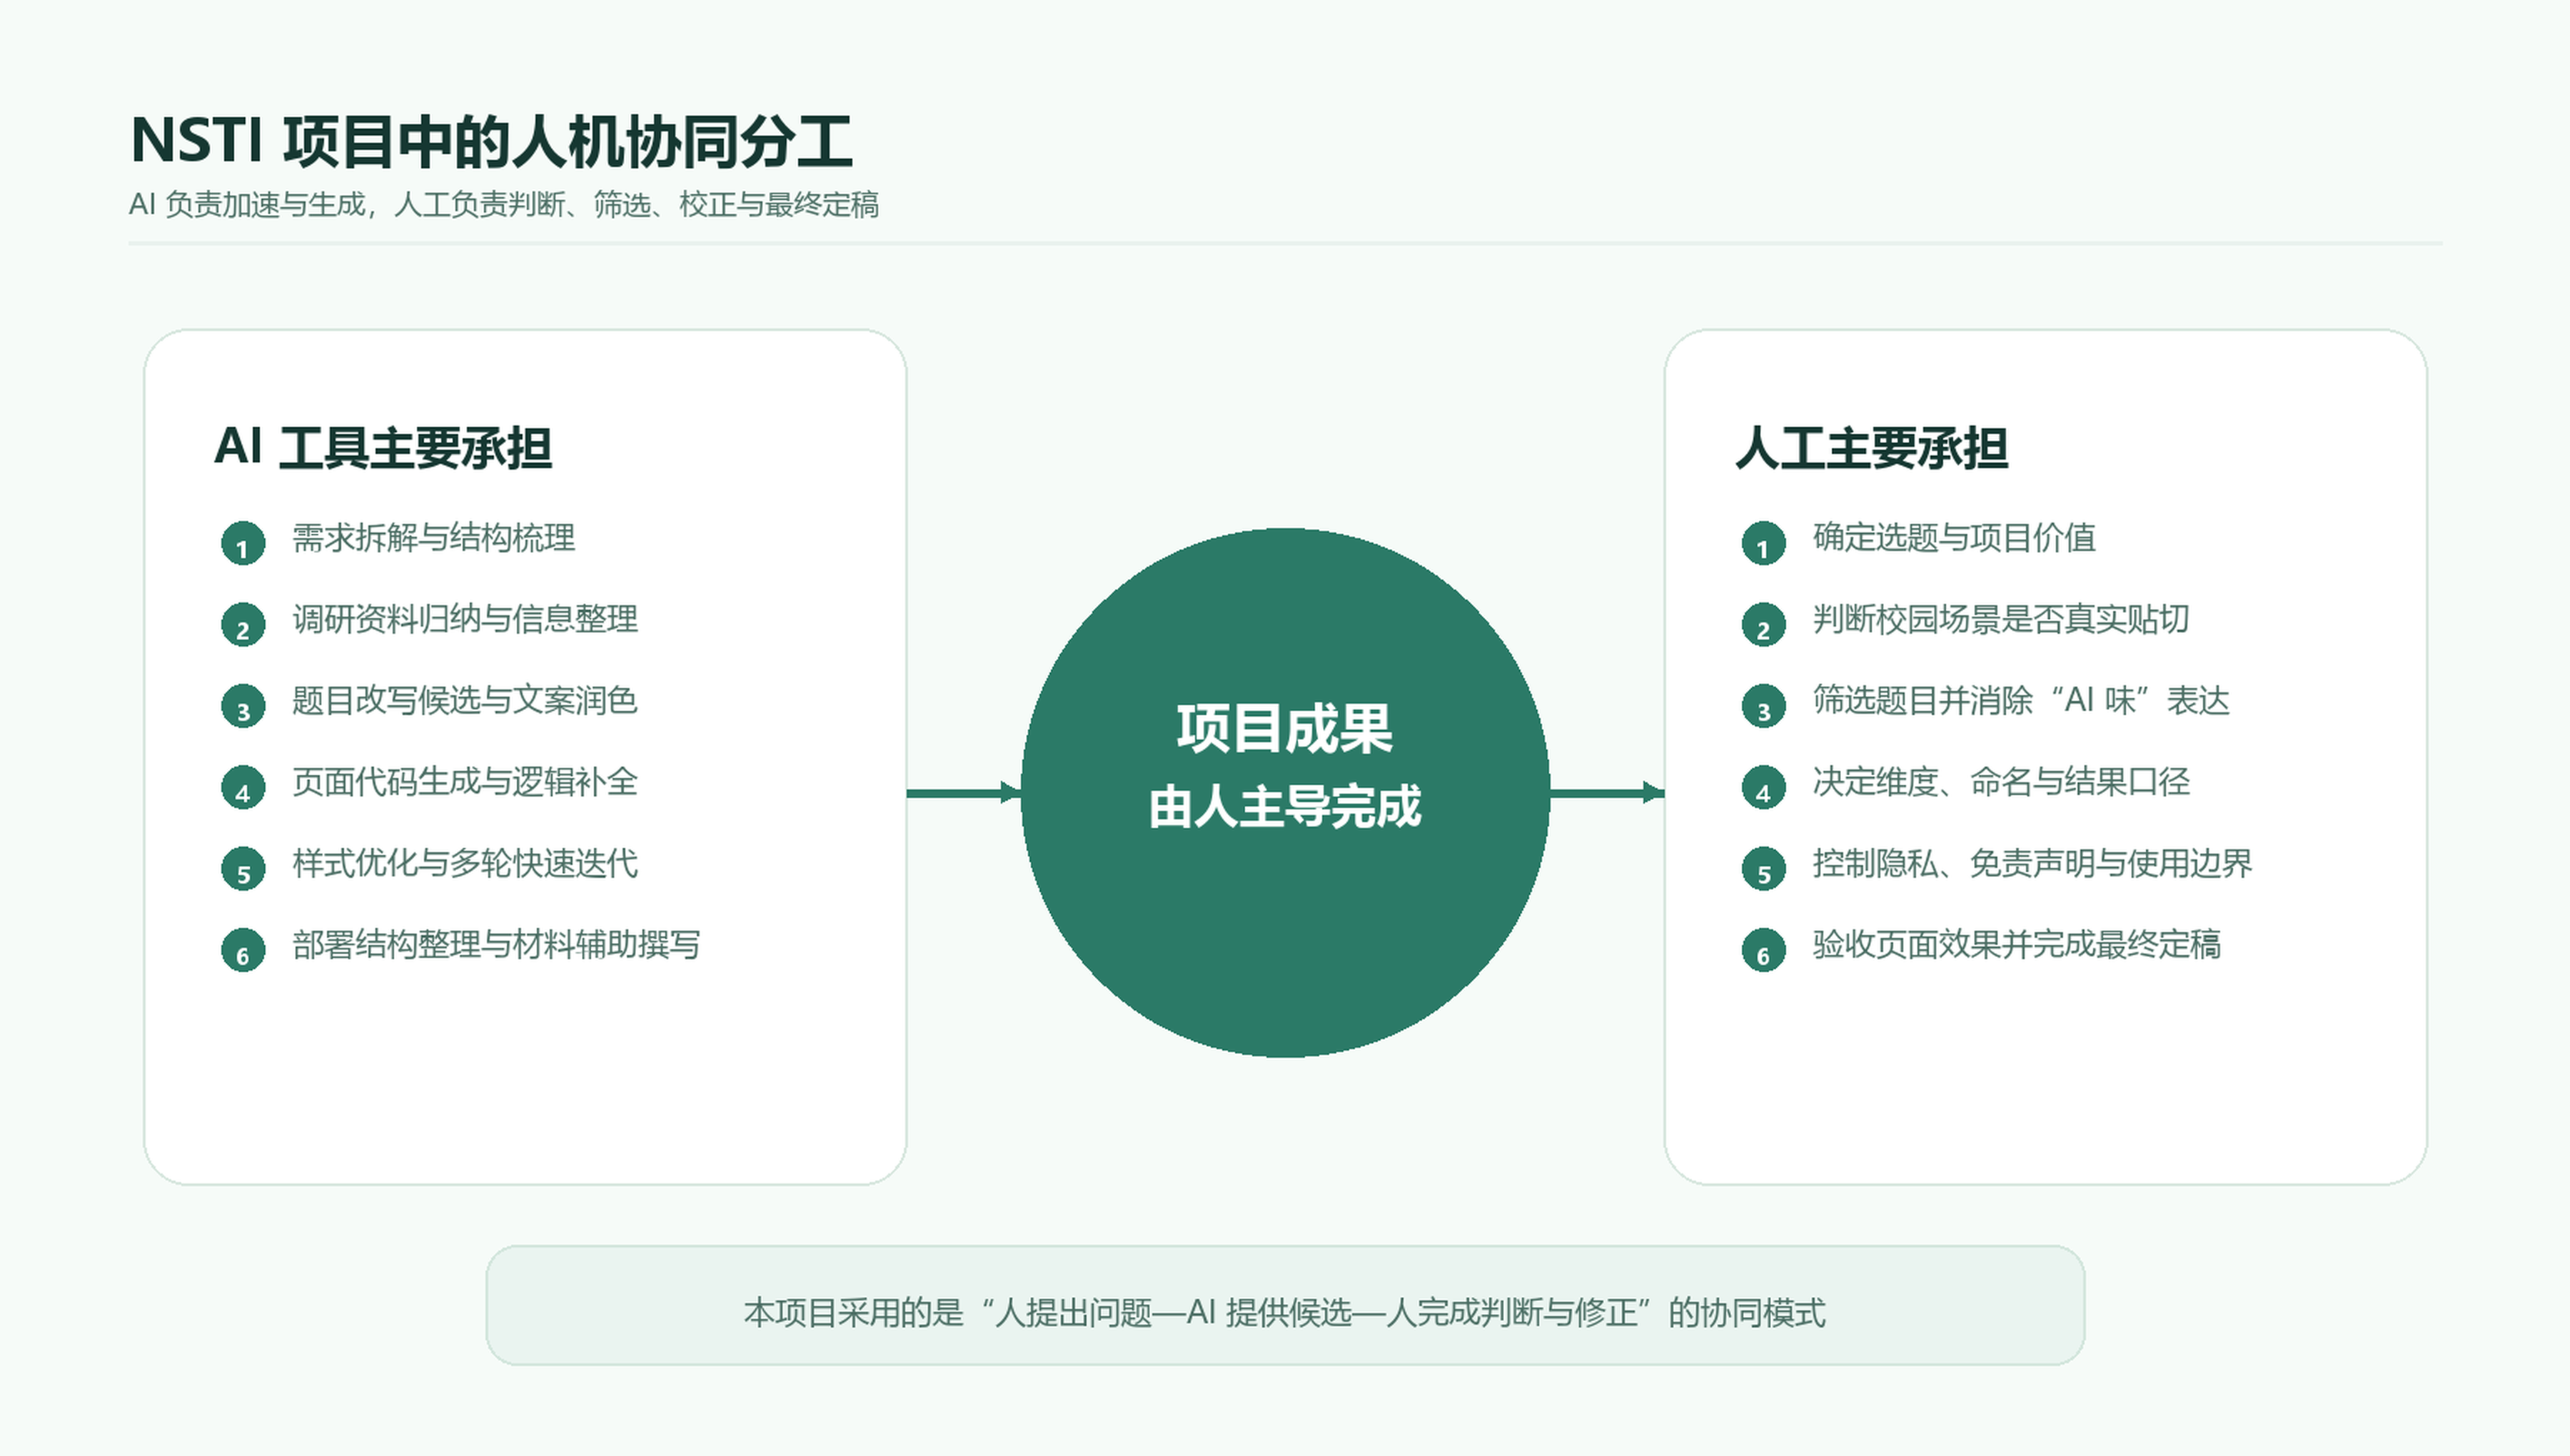
\includegraphics[width=\textwidth]{fig3_collaboration_hires.png}
  \caption{NSTI 项目中的人机协同分工}
\end{figure}

\section{项目成果}

截至目前，NSTI 已形成以下成果：

\begin{enumerate}
  \item 一套校园化偏好测评体系：包括 4 组偏好维度、24 道正式题目、16 类结果卡，以及对应的校园锚点和场景化解释。
  \item 一套完整网页产品原型：包括首页、答题页、结果页、题库说明、评价体系、隐私与免责声明、结果图鉴和随园扩展页面。
  \item 一套文档材料：包括设计构想、题库说明、评价说明、隐私口径、开发说明、材料清单和本 LaTeX 说明文档。
  \item 一个已上线的静态网站：具备前端交互、移动端适配、天气接口和基础访问统计能力。网站访问链接为 \href{https://www.nstitype.xyz}{https://www.nstitype.xyz}。目前网站累计访问量已接近 1000 次，说明它已经不只是本地演示页面，也具备了一定的真实传播和展示效果。
\end{enumerate}

\begin{figure}[H]
  \centering
  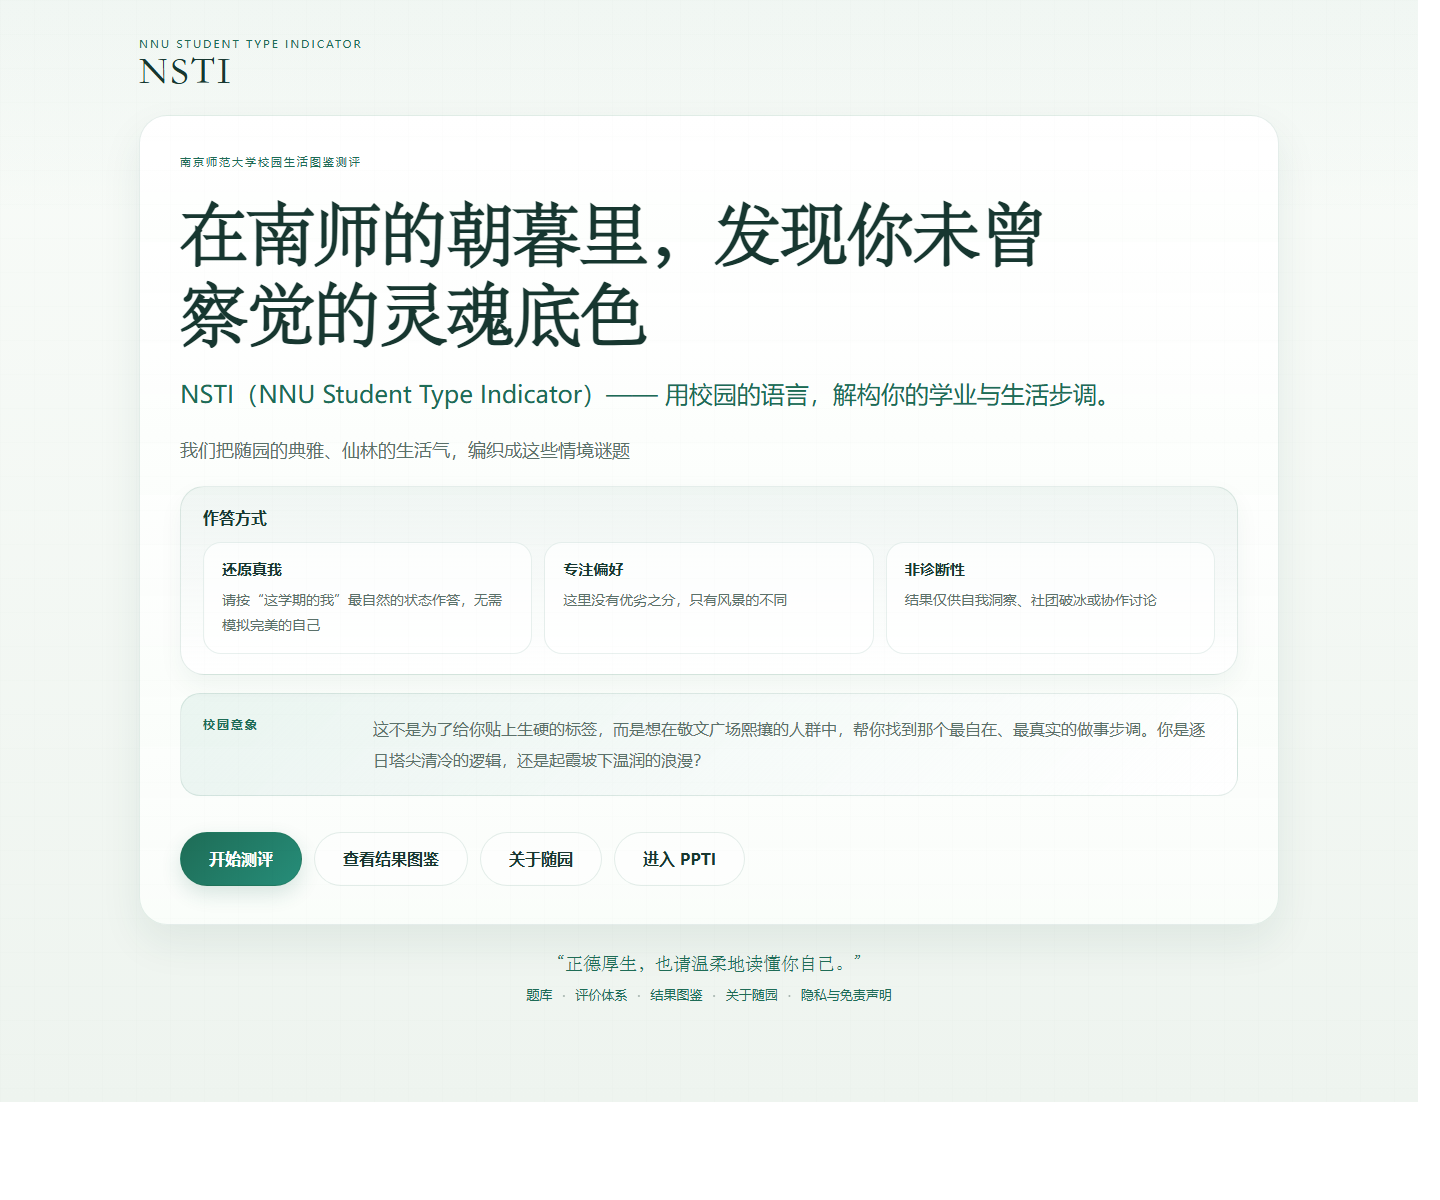
\includegraphics[width=0.92\textwidth]{fig7_homepage.png}
  \caption{NSTI 网站首页实际效果}
\end{figure}

\section{AI 工具的实际价值}

做完 NSTI 之后，我对 AI 工具的价值有了更实际的体会。

前期查资料时，AI 的帮助主要体现在“先把材料理顺”。面对公开资料、题库样本和概念框架时，它可以先做粗整理，我再判断哪些内容值得继续深入，哪些只适合作为参考。

它也明显缩短了从想法到原型的距离。过去从一个项目想法到可运行网页，需要跨过较高的前端门槛；这次我更多是先用自然语言表达需求和限制，再让 Codex 这类 agent 将需求拆成可执行步骤，完成页面结构、交互逻辑、样式调整和文档整理。对我来说，这类工具最直接的价值，是让个人脑子里的创意不再停留在“想一想”的阶段，而是可以被整理成方案、页面、图表和说明材料，逐步变成一个能被他人访问和理解的成果。

它还适合做多轮迭代。题目、结果文案、页面布局都不是一次完成的，而是在“生成、检查、修改、再检查”的循环中慢慢变得可用。

不过，AI 的价值并不等于“自动完成”。在校园化项目里，最重要的判断仍然来自真实经验：哪些场景贴近同学生活，哪些表达看起来通顺但不像本校语境，哪些结果可能被误解。这些问题不能只交给模型。

\section{案例反思与总结}

NSTI 不是一个单纯的代码生成练习，而是一项贯穿问题提出、资料调研、题库搭建、评价体系设计、页面开发、上线部署和材料整理的项目型学习实践。

这次实践让我确认了一点：AI agent 很适合加快进度，却不能替代最终判断。OpenAI Codex 的优势在于可以真正进入项目现场，按我的自然语言说明去改文件、跑脚本、编译材料；但项目真正能不能成立，仍然取决于人的判断。尤其是 NSTI 这种带有校园语境的作品，越到后期，越需要人工把关细节。

因此，我对本项目的人机协同关系的理解是：人负责提出问题、创意和边界；通用模型帮助把自然语言想法整理成更准确的提示词；Codex 作为编辑器 agent 负责把提示词落实到代码、文档和配图中；最后仍由人完成筛选、校正和验收。NSTI 能够从一个初步想法发展为可访问、可展示、可提交的完整项目，正是这种协作方式的结果。

\end{document}
